\documentclass{beamer}

\usepackage[utf8]{inputenc}
\usepackage{default}
\usepackage{amsmath}
\usepackage{upgreek}

\title{Konstruksjon av høydimensjonale nevralt nettverk-potensialer for molekylærdynamikk}
\author{John-Anders Stende}
\institute{
  Fysisk institutt \\
  Universitetet i Oslo
}
\date{Masterpresentasjon, oktober 2017}
\subject{Computational physics}

\AtBeginSection[]
{
  \begin{frame}
    \frametitle{Table of Contents}
    \tableofcontents[currentsection]
  \end{frame}
}

\begin{document}

\frame{\titlepage}

\section{Molekylærdynamikk}

\begin{frame}

\begin{block}{Hva er molekylærdynamikk?}
  \begin{itemize}
  \item Numerisk metode for å simulere atomers og molekylers bevegelser i gasser, væsker og faste stoffer.
  \item Virtuelt eksperiment.
  \end{itemize}
\end{block}

\end{frame}


\begin{frame}

\begin{block}{Dynamikk}
  \begin{itemize}
  \item Partiklenes interaksjoner styrer dynamikken.
  \item Interaksjonene bestemmes av et kraftfelt $\mathbf{F}$:
    \begin{equation*}
    \mathbf{F} = -\nabla V(\mathbf{r})
    \end{equation*}
  \item Potensiell energiflate / potensial):
    \begin{equation*}
      V(\mathbf{r}), \quad \mathbf{r} = (\mathbf{r}_1, \mathbf{r}_2, \cdots, \mathbf{r}_N)
    \end{equation*}
  \item $V(\mathbf{r})$ inneholder all fysikken. 
  \end{itemize}
\end{block}

\end{frame}


\begin{frame}

\begin{columns}[T] % contents are top vertically aligned
  \begin{column}[T]{0.5\linewidth} % each column can also be its own environment
    \begin{block}{Ab inito molekylærdynamikk}
    Løse Schrödinger-likningen ved hvert tidssteg.
    \end{block}
  \end{column}
  \begin{column}[T]{0.5\linewidth} % alternative top-align that's better for graphics
    \begin{block}{Klassisk molekylærdynamikk}
    Bruke en predefinert analytisk funksjon.
    \end{block}
  \end{column}
\end{columns}

\end{frame}


\begin{frame}

\begin{block}{Klassisk potensial}
  \begin{equation*}
  V(\mathbf{r}) \approx \sum_i^N V_1(\mathbf{r}_i) + \sum_{i,j}^N V_2(\mathbf{r}_i, \mathbf{r}_j) + 
  \sum_{i,j,k}^N V_3(\mathbf{r}_i, \mathbf{r}_j, \mathbf{r}_k) + \dots
  \end{equation*}
\end{block}

\begin{block}{Hvordan bør leddene se ut?}
Eksperiementer / kvantemekanikk
\end{block}

\end{frame}


\begin{frame}

\begin{block}{''Fysisk'' strategi:}
 \begin{enumerate}
  \item Starte med en funksjonsform med noen parametre.
  \item Bestemme parametre fra eksperimentelle data.
 \end{enumerate}
\end{block}

\begin{block}{''Matematisk'' strategi:}
 \begin{enumerate}
  \item Produsere kvantemekaniske data. 
  \item Tilpasse en generell funksjonsform til dataene.
 \end{enumerate}
\end{block}

\end{frame}


\begin{frame}
 
\begin{block}{Interpolere datasett}
 \begin{itemize}
  \item Spliner
  \item Minste kvadraters metode
  \item Maskinlæring
 \end{itemize}
\end{block}
 
\end{frame}


\section{Nevrale nettverk}

\begin{frame}
 
\includegraphics[width=0.9\linewidth]{../Figures/Theory/MachineLearningDiagram.png}

\end{frame}


\begin{frame}

\begin{block}{Kunstige nevrale nettverk}
 \begin{itemize}
  \item Etterlikne en biologisk hjerne
  \item Nettverk av matematiske nevroner
 \end{itemize}
\end{block}


\end{frame}


\begin{frame}
 
\centering
\includegraphics[width=0.8\linewidth]{../Figures/Theory/neuron_anatomy.jpg} 

\includegraphics[width=0.8\linewidth]{../Figures/Theory/neuron.pdf} 

\end{frame}


\begin{frame}

\centering
\includegraphics[width=0.8\linewidth]{../Figures/Theory/neuron.pdf} 

\begin{equation*}
 y = f\left(\sum_{i=1}^n w_ix_i + b_i\right) = f(u)
\end{equation*}
 
\end{frame}


\begin{frame}
 
\centering
\includegraphics[width=0.9\linewidth]{../Figures/Theory/networkGeneralAltered.pdf}

\end{frame}


\begin{frame}
 
\centering
\includegraphics[width=0.8\linewidth]{../Figures/Theory/networkWithNotationAltered.pdf}

\begin{equation*}
 y_i^1 = f_1(u_i^1) = f_1\left(\sum_{j=1}^2 w_{ij}^1 x_j  + b_i^1\right)
\end{equation*}

\end{frame}


\begin{frame}

\begin{equation*}
  y_1^3 = f_3\left[\sum_{j=1}^3 w_{1j}^3 f_2\left(\sum_{k=1}^3 w_{jk}^2 f_1\left(\sum_{m=1}^2 w_{km}^1 x_m + b_k^1\right) + b_j^2\right)
  + b_1^3\right]
\end{equation*}
\begin{equation*}
 h(x) = c_1 f(c_2 x + c_3) + c_4
\end{equation*}
\centering
\includegraphics[width = 0.7\linewidth]{../Figures/Theory/activationFlex.pdf}

\end{frame}
 
 
\begin{frame}{Matrix notation}

\begin{equation*}
  y_i^2 = f_2\left(\sum_{j=1}^3 w_{ij}^2 y_j^1 + b_i^2\right)
\end{equation*}
\begin{equation*}
 \mathbf{y}_2 = f_2(\mathrm{W}_2 \mathbf{y}_{1} + \mathbf{b}_{2}) = 
 f_2\left(\left[\begin{array}{ccc}
    w^2_{11} &w^2_{12} &w^2_{13} \\
    w^2_{21} &w^2_{22} &w^2_{23} \\
    w^2_{31} &w^2_{32} &w^2_{33} \\
    \end{array} \right] \cdot
    \left[\begin{array}{c}
           y^1_1 \\
           y^1_2 \\
           y^1_3 \\
          \end{array}\right] + 
    \left[\begin{array}{c}
           b^2_1 \\
           b^2_2 \\
           b^2_3 \\
          \end{array}\right]\right)
\end{equation*}

\end{frame}


\begin{frame}{Activation functions}

\begin{columns}[T] % contents are top vertically aligned

 \begin{column}[T]{0.5\linewidth} % each column can also be its own environment
  The sigmoid
  \begin{equation*}
  f(x) = \frac{1}{1 + e^{-x}}
  \label{sigmoidActivationFunction}
  \end{equation*}
  and the hyperbolic tangent
  \begin{equation*}
  f(x) = \tanh(x)
  \label{tanhActivationFunction}
  \end{equation*}
 \end{column}
 
 \begin{column}[T]{0.5\linewidth} % alternative top-align that's better for graphics
  \centering
  \includegraphics[width=\linewidth]{../Figures/Theory/activationFunctionsAltered.pdf}
 \end{column}
 
\end{columns}
  
\end{frame}


\begin{frame}
 
\centering
\includegraphics[width=0.9\linewidth]{../Figures/Presentation/interpolation.pdf}
\begin{block}{Regresjon med nevralt nettverk}
 \begin{itemize}
  \item Regresjon: Interpolere datasett $\mathrm{X} \rightarrow \mathrm{Y}$
  \item $X$: inputdata, $Y$: outputdata, $X_{i*}$: treningseksempel. 
  \item Trening: Iterativt minimere feilen til et sett med kjente energier. 
 \end{itemize}
\end{block}

\end{frame}


\begin{frame}
 
\begin{block}{Feilen defineres ved en cost-funksjon:} 
 \begin{equation*}
 \Gamma = \Gamma\bigr(\{\mathrm{W}_l\}, \{\mathbf{b}_l\}, \mathrm{X}, \mathrm{Y}\bigr)
        = \frac{1}{2N}\sum_{i=1}^N (Y_i - y_i)^2
 \end{equation*}
\end{block}

\begin{block}{Optimering med gradient descent:}
 \begin{equation*}
  \mathbf{\uptheta}_{k+1} = \mathbf{\uptheta}_{k} - \gamma \nabla_{\mathbf{\uptheta}_k} \Gamma(\mathbf{\uptheta})
 \end{equation*}
 Mange forskjellige måter å justere $\gamma$ på. 
\end{block}

\end{frame}


\begin{frame}{Hvordan finne gradienten av nettet?}
 
\centering
\includegraphics[width = 0.8\linewidth]{../Figures/Theory/backprop.pdf}

\begin{block}{Backpropagation}
 \begin{enumerate}
  \item Sender hvert treningsseksempel gjennom nettet. 
  \item Output (energi) sammenliknes med kjent energi. 
  \item Feilen propagares \textit{bakover} ved kjerneregelen og vektene justeres. 
 \end{enumerate}
\end{block}
 
\end{frame}

\section{Nevralt nettverk-potensial}

\begin{frame}
 
\begin{block}{Flere muligheter}
 \begin{itemize}
  \item Et eller flere nettverk? 
  \item Hvordan representere energien?
 \end{itemize}
\end{block}

\begin{block}{Behler-Parrinello-metoden}
 \begin{equation*}
       E = \sum_{i=1}^N E_i
 \end{equation*}
 \begin{itemize}
  \item Atomsentrert: Hver atomenergi $E_i$ avhenger av alle naboatomer opp til en cutoff $r_c$.
  \item Hvert atom har et eget nettverk og et sett av symmetrifunksjoner som beskriver cutoff-kulen. 
  \item Hver atomtype har identiske nettverk og symmetryfunskjonssett.  
 \end{itemize}
\end{block}

\end{frame}


\begin{frame}

\begin{columns}[c] % contents are top vertically aligned
  \begin{column}[c]{0.4\linewidth} % each column can also be its own environment
   \centering
   \includegraphics[width=\linewidth]{../Figures/Presentation/cutoffSphere.pdf}
  \end{column}
  \begin{column}[c]{0.6\linewidth} % alternative top-align that's better for graphics
   \includegraphics[width=\linewidth]{../Figures/Presentation/BehlerParrinello.pdf}
  \end{column}
\end{columns}

Gjøre om slik at bare G- og NN-bokstavene er i farger, ikke selve kulene. 
Det er symmetrivektorene og NN-ene som er like, ikke selve posisjonene osv. 

\end{frame}










\end{document}
